\documentclass{beamer}

%\usepackage[utf8]{inputenc} % set input encoding (not needed with XeLaTeX)
\usepackage[portuguese]{babel}
%\usepackage{fontspec}

%\usepackage{fontspec}
%\setmainfont{Minion Pro}

\usetheme{metropolis}

\usepackage{polyglossia}
\setmainlanguage{portuges}

%\usecolortheme{seahorse}

\usepackage{graphicx} % support the \includegraphics command and options

% \usepackage[parfill]{parskip} % Activate to begin paragraphs with an empty line rather than an indent

%%% PACKAGES
%\usepackage{booktabs} % for much better looking tables
%\usepackage{array} % for better arrays (eg matrices) in maths
%\usepackage{tabu}
%\usepackage{colortbl}
%\usepackage{paralist} % very flexible & customisable lists (eg. enumerate/itemize, etc.)
%\usepackage{verbatim} % adds environment for commenting out blocks of text & for better verbatim
\usepackage{float}
%\usepackage{subfig} % make it possible to include more than one captioned figure/table in a single float
%\usepackage{makeidx} % makes index
\usepackage{hyperref} % TOC clicável
%\usepackage{csquotes}
\usepackage[font={small,it}]{caption}
\usepackage{tikz} % matrizes
\usepackage{pgfplots}
\pgfplotsset{compat=1.12}
%\usepackage[numbers]{natbib} %citações

%\usepackage{algorithm} % pseudocode
%\usepackage{algpseudocode}

% the following is needed for syntax highlighting
\usepackage{color}

\definecolor{purple}{RGB}{90, 10, 132}

\hypersetup{
    colorlinks,
    citecolor=purple,
    filecolor=purple,
    linkcolor=purple,
    urlcolor=purple
}

\beamertemplatenavigationsymbolsempty

\makeatletter
\newlength\beamerleftmargin
\setlength\beamerleftmargin{\Gm@lmargin}
\makeatother

\newcommand{\lmr}{\fontfamily{lmr}\selectfont} % Latin Modern Roman
\renewcommand{\inserttitle}{aaa}

%%% END Article customizations

%%% The "real" document content comes below...

\title{LabHacker}
\subtitle{Laboratório Brasileiro de Cultura Digital}
\author{Erin Pinheiro Manal - Feiticeira Tecnológica}
%\date{} % Activate to display a given date or no date (if empty),
         % otherwise the current date is printed 

\begin{document}
\begin{frame}
  \begin{tikzpicture}[remember picture,overlay]
    \node [anchor=north west,xshift=-0.125cm,yshift=0.125cm] at (current page.north west) {
      
\includegraphics[width=\paperwidth]{banner-lab}
    };
  \end{tikzpicture}
\begin{minipage}[b][\paperheight]{\textwidth}
    \vfill%
    \vspace{2.5em}
    \ifx\insertsubtitle\@empty\else\usebeamertemplate*{subtitle}\fi
    \usebeamertemplate*{title separator}
    \ifx\beamer@shortauthor\@empty\else\usebeamertemplate*{author}\fi
    \ifx\insertdate\@empty\else\usebeamertemplate*{date}\fi
    \ifx\insertinstitute\@empty\else\usebeamertemplate*{institute}\fi
    \vfill
    \vspace*{1mm}
\end{minipage}
\end{frame}

\begin{frame}
  \frametitle{Quem sou eu?}
  \centering
    \begin{tikzpicture}
      \clip (0,0) circle (2.5cm) node {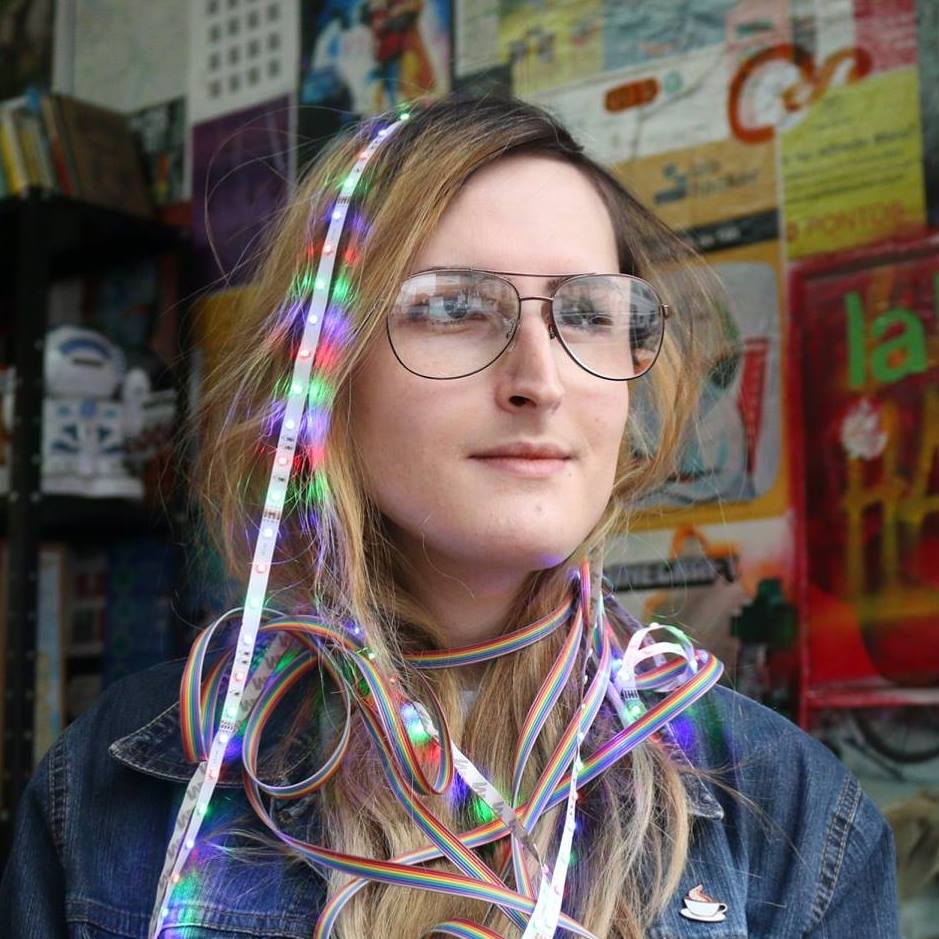
\includegraphics[width=.5\linewidth]{erin}};
    \end{tikzpicture}
  \par
  \textbf{Erin Pinheiro Manal} - Feiticeira Tecnológica do LabHacker
  Estudante de Sistemas de Informação - EACH-USP
\end{frame}

\begin{frame}
  \frametitle{Quem sou eu?}
  \begin{columns}
    \begin{column}{0.5\textwidth}
      O que faz uma feiticeira tecnológica?
    \end{column}
    \begin{column}{0.5\textwidth}
      \begin{tikzpicture}[remember picture,overlay]
        \node[anchor=south east,xshift=1em,yshift=-.2em] at (current page.south east) {
          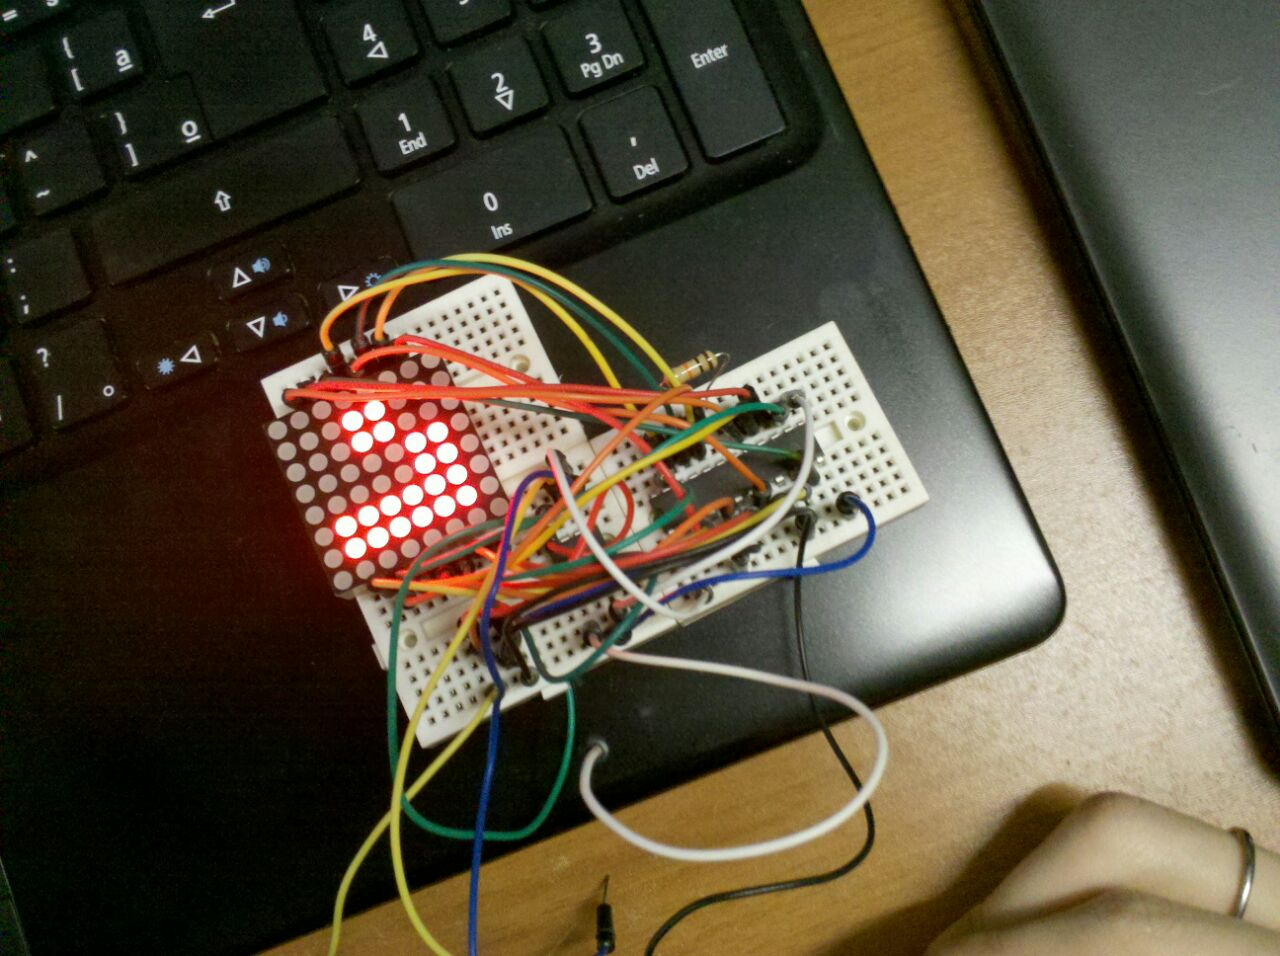
\includegraphics[trim=280 0 110  0,clip,height=\textheight]{feiticos}
        };
      \end{tikzpicture}
    \end{column}
  \end{columns}
\end{frame}

\begin{frame}
  \frametitle{Quem sou eu?}
  \centering
  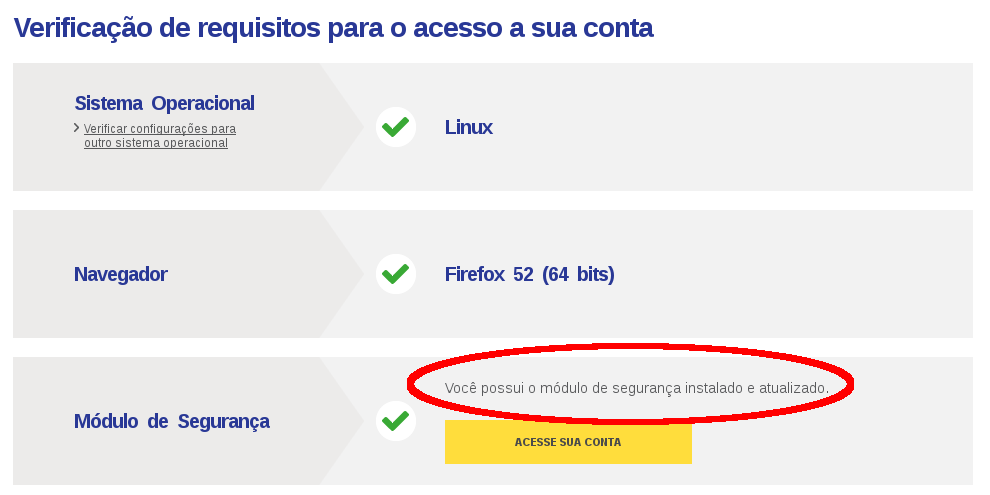
\includegraphics[width=\linewidth]{modulobb}
\end{frame}

\begin{frame}
  \frametitle{O que é cultura hacker?}
  \begin{columns}
    \begin{column}{0.5\textwidth}
      \begin{itemize}
        \item \textbf{Como surgiu?}
      \end{itemize}
      Tech Model Railroad Club - MIT
      \begin{itemize}
        \item Berço da cultura hacker
        \item Utilizaram relês de telefone para controlar os trens
      \end{itemize}
      \vspace*{\baselineskip}
    \end{column}
    \begin{column}{0.5\textwidth}
      \begin{tikzpicture}[remember picture,overlay]
        \node[anchor=south east,xshift=0.125cm,yshift=-0.125cm] at (current page.south east) {
          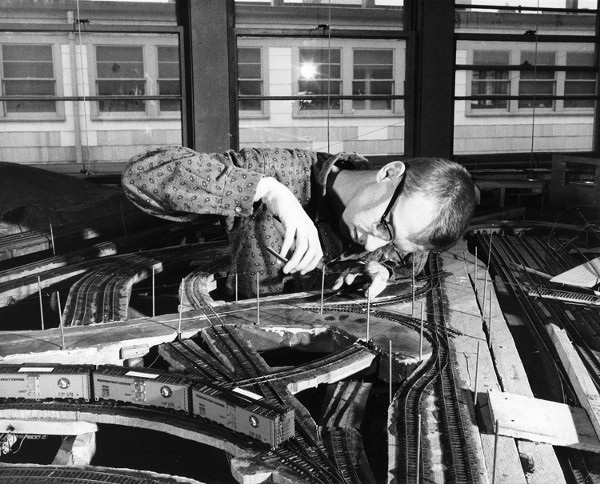
\includegraphics[trim=110 0 60  0,clip,height=\textheight]{tmrc}
        };
      \end{tikzpicture}
    \end{column}
  \end{columns}
\end{frame}

\begin{frame}
  \frametitle{O que é cultura hacker?}
  \begin{columns}
    \begin{column}{0.5\textwidth}
      \begin{itemize}
        \item Como surgiu?
        \item \textbf{O que significa?}
      \end{itemize}
      Em resumo, modificar o propósito de algo que já existe
      \vspace*{3\baselineskip}
    \end{column}
    \begin{column}{0.5\textwidth}
      \begin{tikzpicture}[remember picture,overlay]
        \node[anchor=south east,xshift=0.125cm,yshift=-0.125cm] at (current page.south east) {
          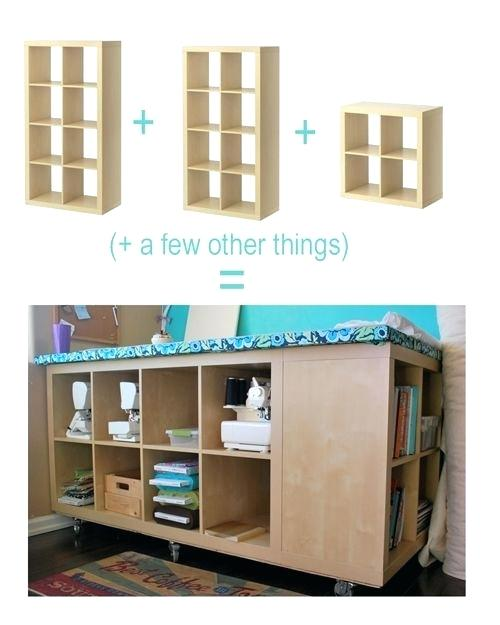
\includegraphics[height=\textheight]{ikeahack}
        };
      \end{tikzpicture}
    \end{column}
  \end{columns}
\end{frame}

\begin{frame}
  \frametitle{O que é cultura hacker?}
  \begin{columns}
    \begin{column}{0.5\textwidth}
      \begin{itemize}
        \item Como surgiu?
        \item O que significa?
        \item \textbf{O que eu entendo por isso?}
      \end{itemize}
      Trazer alguma mudança para um processo, uma situação, um mecanismo, etc...
    \end{column}
    \begin{column}{0.5\textwidth}
      \begin{tikzpicture}[remember picture,overlay]
        \node[anchor=south east,yshift=-0.125cm] at (current page.south east) {
          
\includegraphics[height=\textheight]{captunderpants}
        };
      \end{tikzpicture}
    \end{column}
  \end{columns}
\end{frame}

\begin{frame}
  \frametitle{O que o lab faz?}
  \hspace*{-\beamerleftmargin}%
  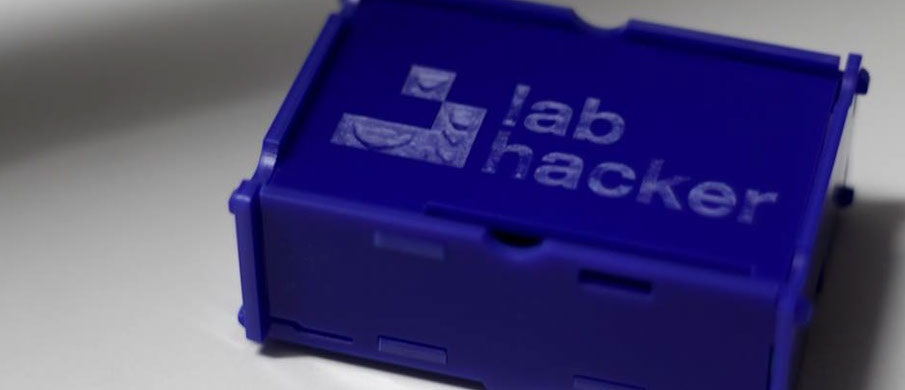
\includegraphics[width=\paperwidth]{labcaixinha}
\end{frame}

\begin{frame}
  \frametitle{Ônibus Hacker}
  \begin{columns}
    \begin{column}{0.5\textwidth}
      * 2014 - † 2018
      \begin{itemize}
        \item Rodou o país fazendo oficinas
        \item Quebrou várias vezes
        \item Tem mais histórias pra contar do que eu
      \end{itemize}
      \url{http://bit.ly/doc-bus}
    \end{column}
    \begin{column}{0.5\textwidth}
      \begin{tikzpicture}[remember picture,overlay]
        \node[anchor=south east,xshift=0.125cm,yshift=-0.125cm] at (current page.south east) {
          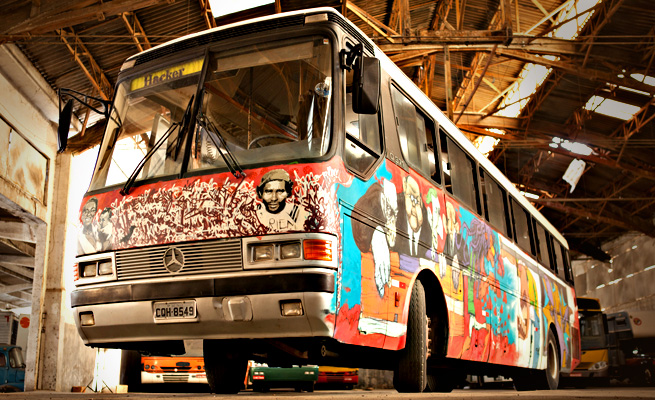
\includegraphics[trim=70 0 250 0,clip,height=\textheight]{onibus}
        };
      \end{tikzpicture}
    \end{column}
  \end{columns}
\end{frame}

\begin{frame}
  \frametitle{Cryptokids}
  \begin{columns}
    \begin{column}{0.5\textwidth}
      Maneira lúdica de se ensinar criptografia para crianças através de uma narratória de detetive
      
      Executada nas CryptoRaves 2016 e 2018
      
      \vspace{\baselineskip}%
      Morsebox:
      \url{http://bit.ly/morsebox}
    \end{column}
    \begin{column}{0.5\textwidth}
      \begin{tikzpicture}[remember picture,overlay]
        \node[anchor=south east,xshift=0.125cm,yshift=-0.125cm] at (current page.south east) {
          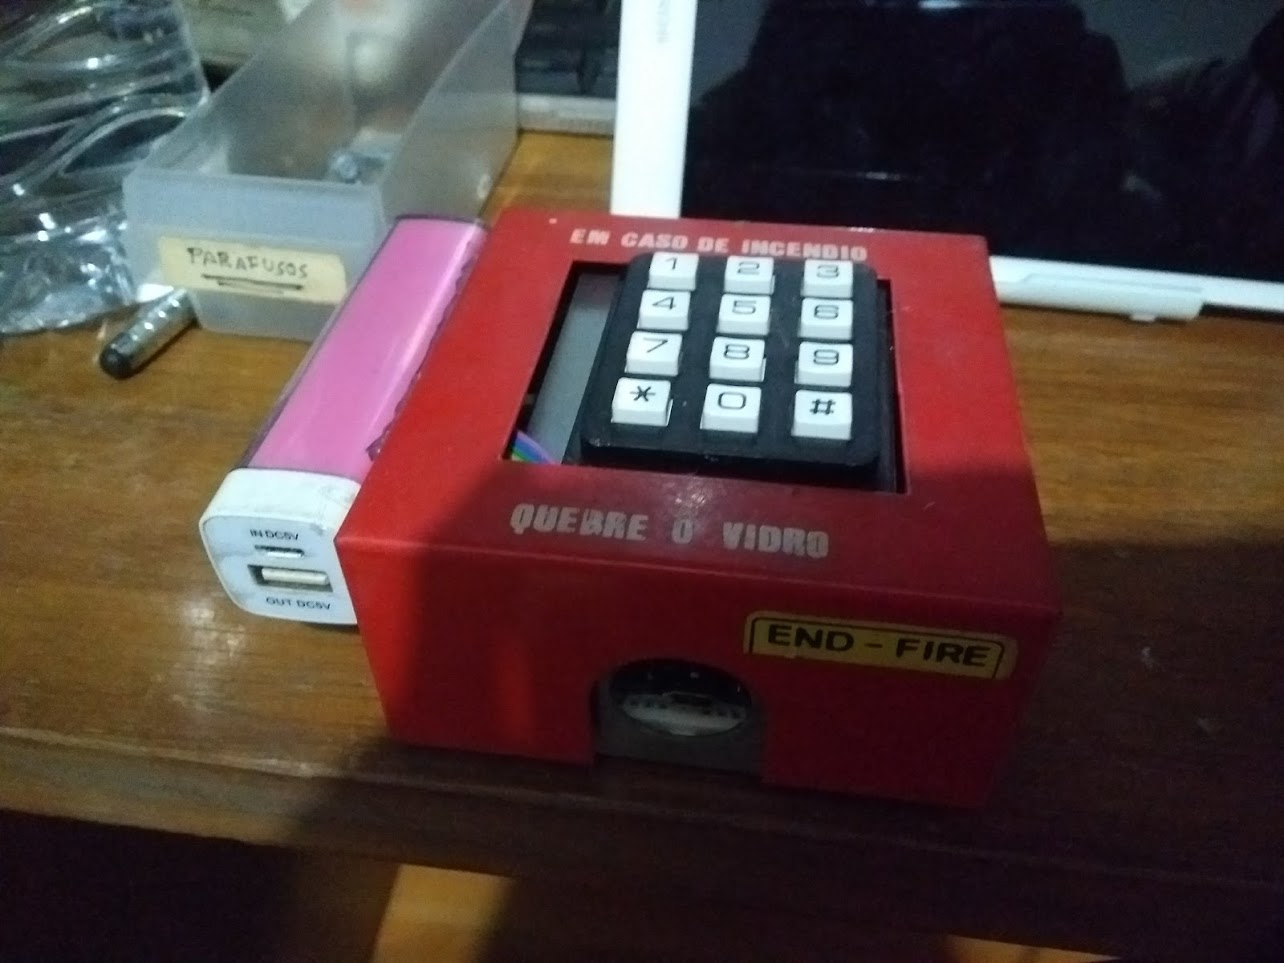
\includegraphics[trim=230 0 270 0,clip,height=\textheight]{morsebox}
        };
      \end{tikzpicture}
    \end{column}
  \end{columns}
\end{frame}

\begin{frame}
  \frametitle{Extrato Parlamentar}
  \begin{columns}
    \begin{column}{0.5\textwidth}
      Máquina que imprime um extrato de todas as PLs em tramitação na câmara naquele dia
      
      \vspace{\baselineskip}%
      \url{https://github.com/LabHackerSP/extrato-parlamentar}
    \end{column}
    \begin{column}{0.5\textwidth}
      \begin{tikzpicture}[remember picture,overlay]
        \node[anchor=south east,xshift=0.125cm,yshift=-0.125cm] at (current page.south east) {
          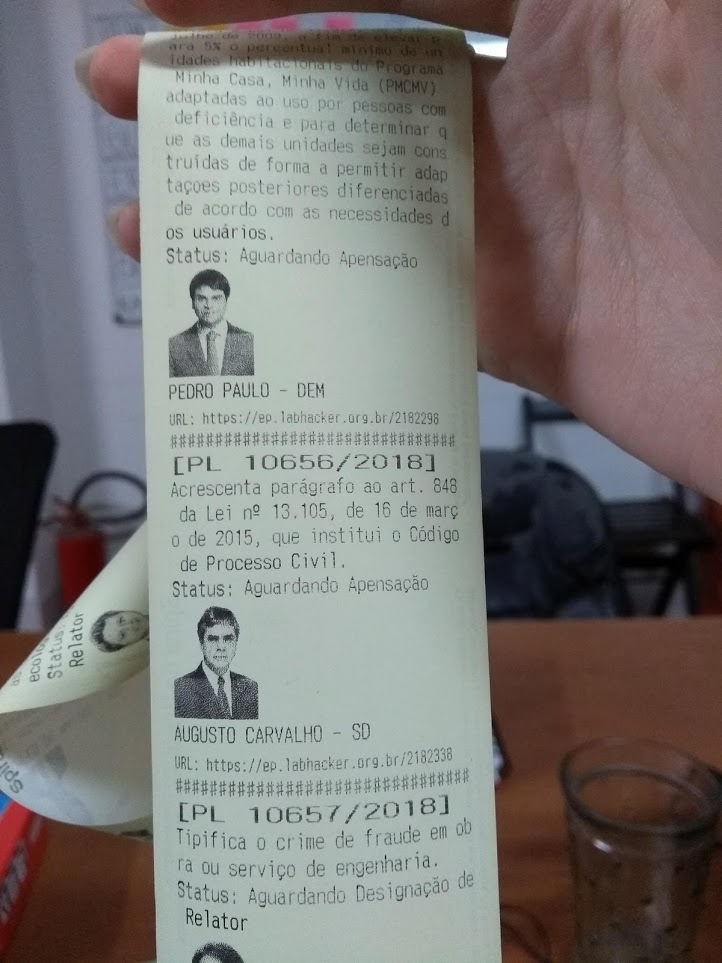
\includegraphics[trim=70 70 70 0,clip,height=\textheight]{extrato}
        };
      \end{tikzpicture}
    \end{column}
  \end{columns}
\end{frame}

\begin{frame}
  \frametitle{SABESPComplex}
  \begin{columns}
    \begin{column}{0.5\textwidth}
      Jogo inspirado em Mu Complex, baseado em informações reais sobre a SABESP e com o intuito de ensinar comandos de terminal ao mesmo tempo
    \end{column}
    \begin{column}{0.5\textwidth}
      \begin{tikzpicture}[remember picture,overlay]
        \node[anchor= east,xshift=0.125cm,yshift=-0.125cm] at (current page.east) {
          
\includegraphics[trim=30 0 30 0,clip,height=0.8\textheight]{sabesp}
        };
      \end{tikzpicture}
    \end{column}
  \end{columns}
\end{frame}

\begin{frame}
  \frametitle{Agenda Pública}
  \begin{columns}
    \begin{column}{0.5\textwidth}
      Aplicativo de celular com datas e horários de eventos oficiais, facilitando a participação pública
    \end{column}
    \begin{column}{0.5\textwidth}
      \begin{tikzpicture}[remember picture,overlay]
        \node[anchor= south east,yshift=-0.125cm] at (current page.south east) {
          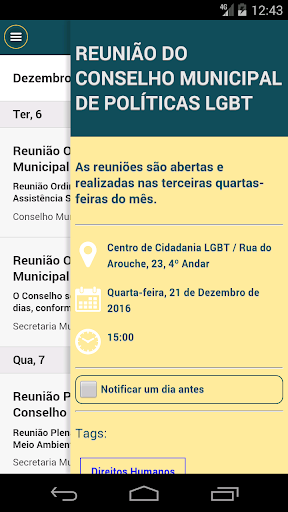
\includegraphics[height=\textheight]{agenda}
        };
      \end{tikzpicture}
    \end{column}
  \end{columns}
\end{frame}

\begin{frame}
  \frametitle{Open Government Partnership}
  \begin{columns}
    \begin{column}{0.5\textwidth}
      Participei do evento da OGP de dezembro de 2016, desenvolvi uma ferramenta para auxiliar na busca de licitações para Spend Network
      
      \vspace{\baselineskip}%
      \url{https://github.com/Lana-chan/opendata}
    \end{column}
    \begin{column}{0.5\textwidth}
      \begin{tikzpicture}[remember picture,overlay]
        \node[anchor= south east,xshift=0.125cm,yshift=-0.125cm] at (current page.south east) {
          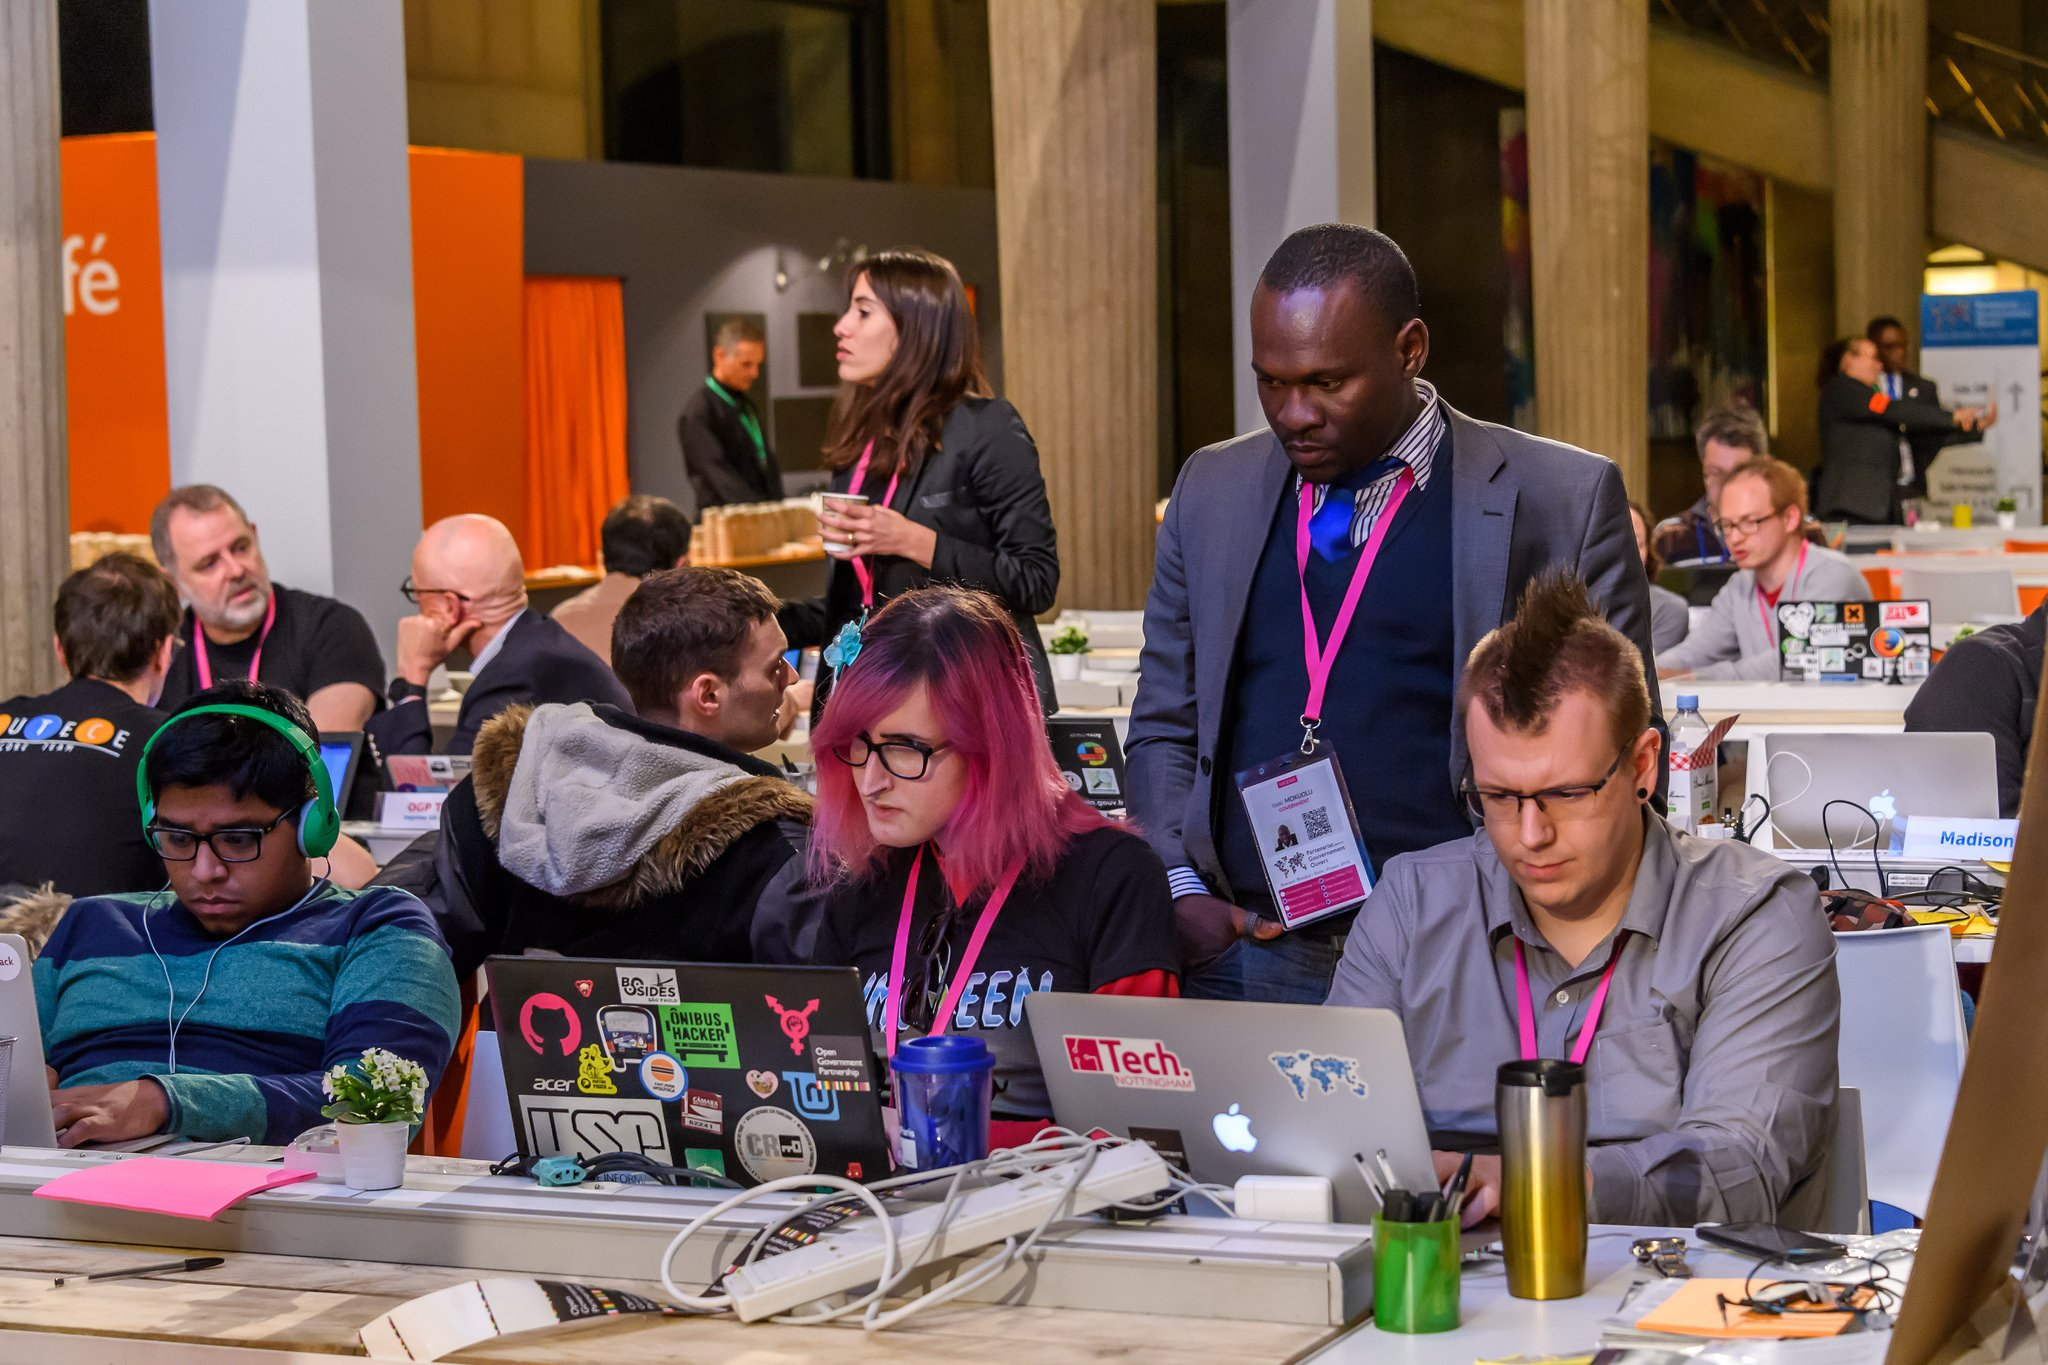
\includegraphics[trim=400 0 600 0,clip,height=\textheight]{ogp}
        };
      \end{tikzpicture}
    \end{column}
  \end{columns}
\end{frame}

\begin{frame}
  \begin{tikzpicture}[remember picture,overlay]
    \node[anchor=north east,xshift=0.125cm,yshift=0.125cm] at (current page.north east) {
      
\includegraphics[width=10em]{forkme}
    };
  \end{tikzpicture}
  \centering \Large
  \textbf{Hackeie esta apresentação \lmr{\LaTeX}!}\par
  \url{https://github.com/LabHackerSP/apresentacao-governo-aberto}
  \bigbreak
  Dúvidas?
\end{frame}

\end{document}
